\documentclass[onecolumn]{article}
\usepackage{graphicx} % Required for inserting images
\usepackage{amsmath}
\usepackage{amsfonts}
\usepackage{pythonhighlight}
\usepackage{datetime}
\usepackage{subcaption}
\usepackage{titling}
\usepackage{enumitem}
\usepackage{matlab-prettifier}
\usepackage{hyperref}
\usepackage[a4paper, total={6in, 8in}]{geometry}

\footskip = 1pt
\textheight = 700pt
\setlength{\droptitle}{-10em}

\title{IN3170 V24 - Lab 3}
\author{Andreas Engøy, Simen Norrud, Erik Røset \& Daniel Tran}
\date{\monthname[\the\month] \the\year}

\begin{document}
\maketitle


\section{Task 1}
\subsection{Equipment}
\begin{table}[h]
    \centering
    \begin{tabular}{|c|c|c|}
        \hline
        \textbf{Component} & \textbf{Model} & \textbf{Quantity} \\
        \hline
        Resistor & 120k$\Omega$ & 1 \\
        Capacitor & 390pF & 3 \\

        \hline
    \end{tabular}
    \caption{List of components used in task 1.}
    \label{tab:bom}
\end{table}



\section{Task 2}
In an ideal current source, the output current is independent of the voltage across the terminals. I.e. the current source maintains the same current throughout the circuit, despite changes to $V_{DS}$.

A Field-Effect Transistor (FET) operating in the saturation region exhibits the same characteristics as an ideal current source. This can be seen from the $I_D$ vs $V_{DS}$ curve in the saturation region, where the current is almost constant. This is because $V_{DS}$ approching the saturation region is high enough that it has maxed out the number of charge carriers that can contribute to current flow, making the gate voltage the primarily factor to the current flow.

In the plot, the curve will flatten out in this region. In a practical FET, the curve will not be completely flat (indicating that the current is not completely constant), but it will give a good approximation of an ideal current source.

\begin{figure}[h!]
    \centering
    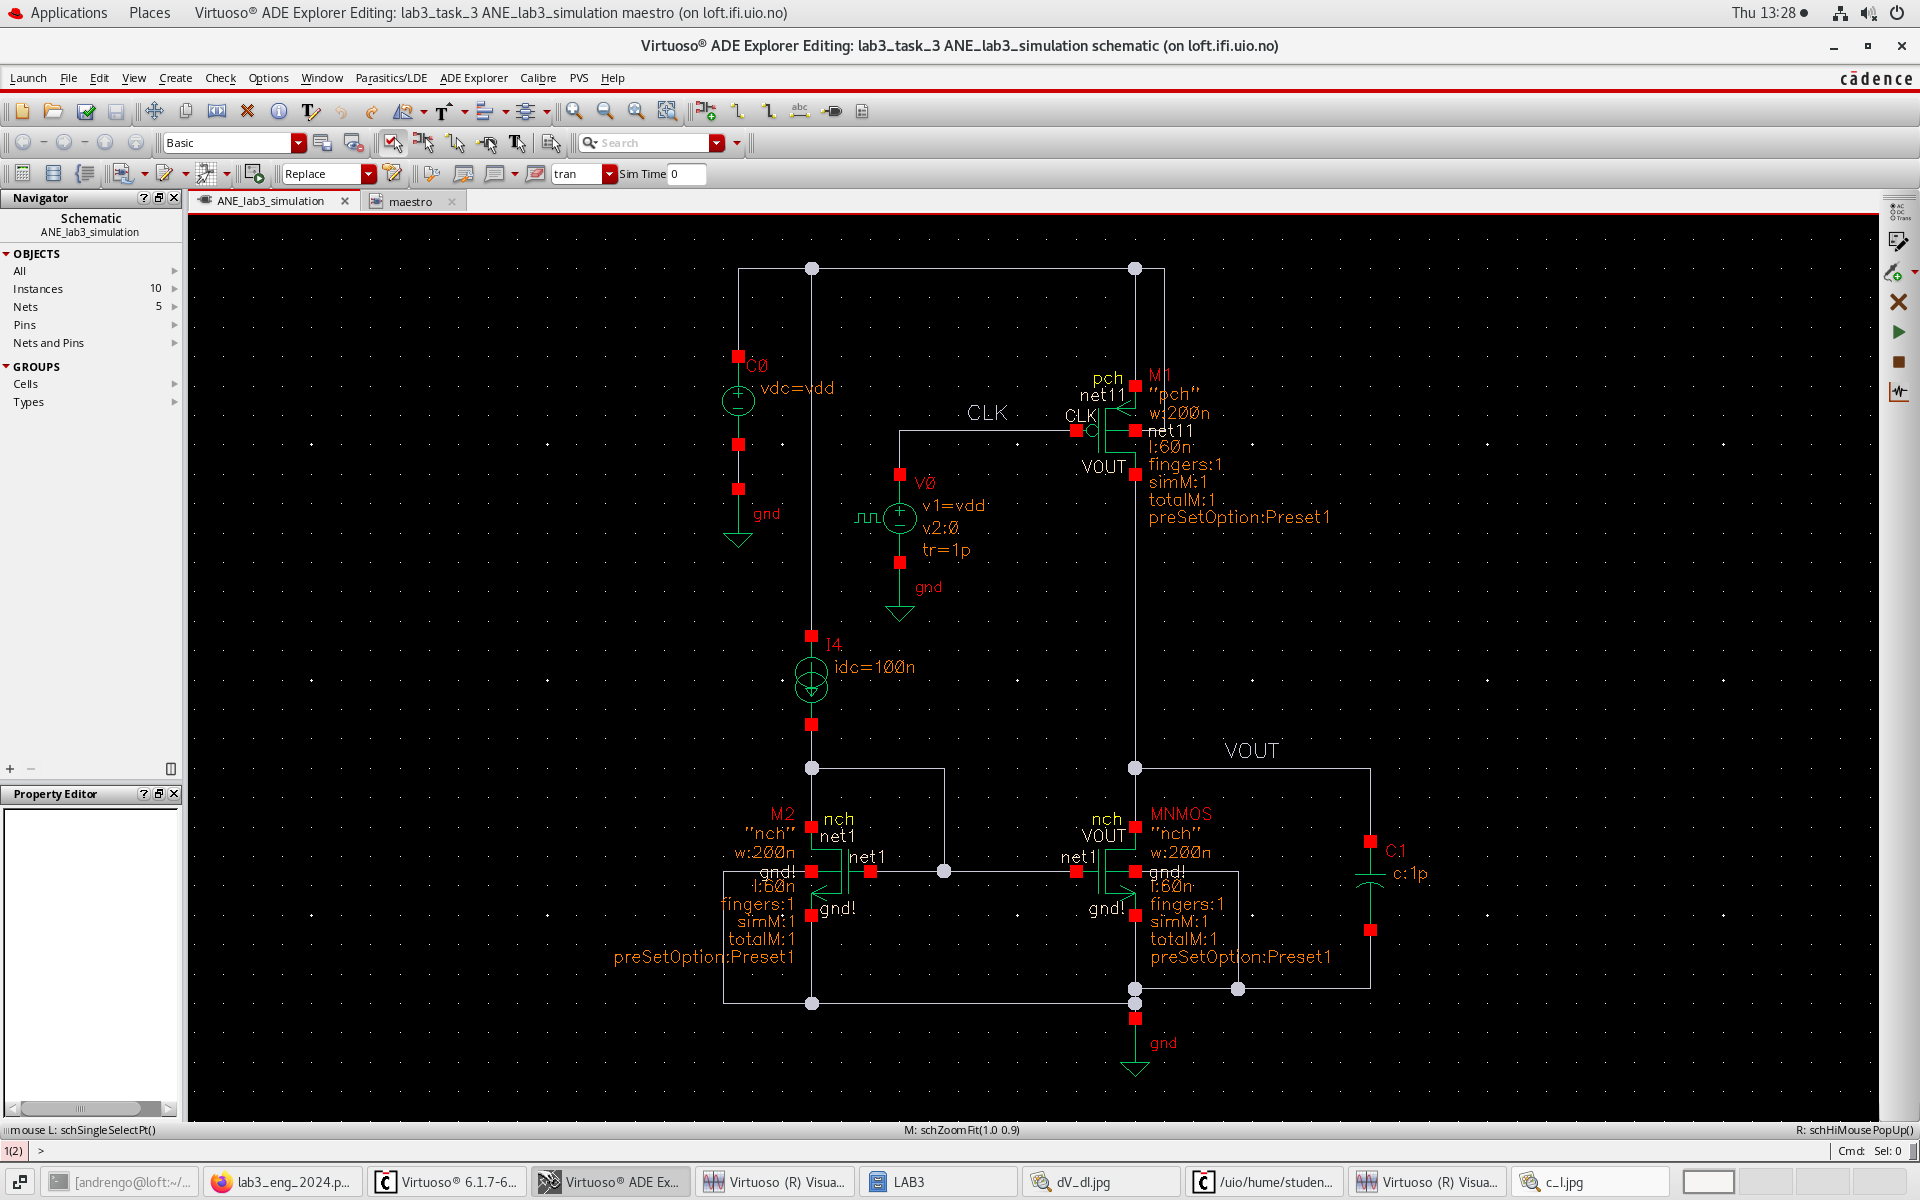
\includegraphics[width=0.8\textwidth]{c).png}
    \caption{Screencapture of the circuit in figure 1 c) from the lab manual simulated in Cadence.}
    \label{fig:circuitc}
\end{figure}

The bias current is implementet as a current mirror, consisting of $M2$ and $I4$, which sets the current that flows through $MNMOS$.

\paragraph*{Adding a voltage cascode}


\begin{figure}[h!]
    \centering
    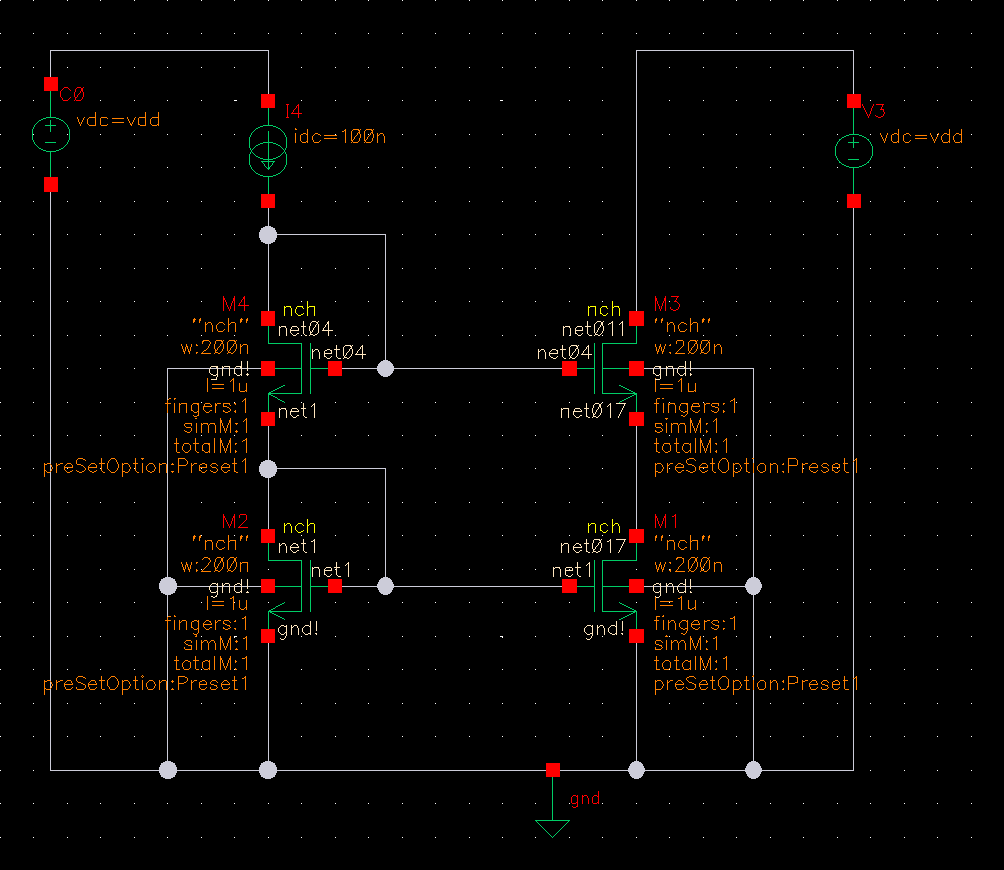
\includegraphics[width=0.8\textwidth]{circuit_d_cascode.png}
    \caption{Screencapture of the circuit in figure 1 d) from the lab manual simulated in Cadence.}
    \label{fig:circuitd}
\end{figure}

\begin{figure}[h!]
    \centering
    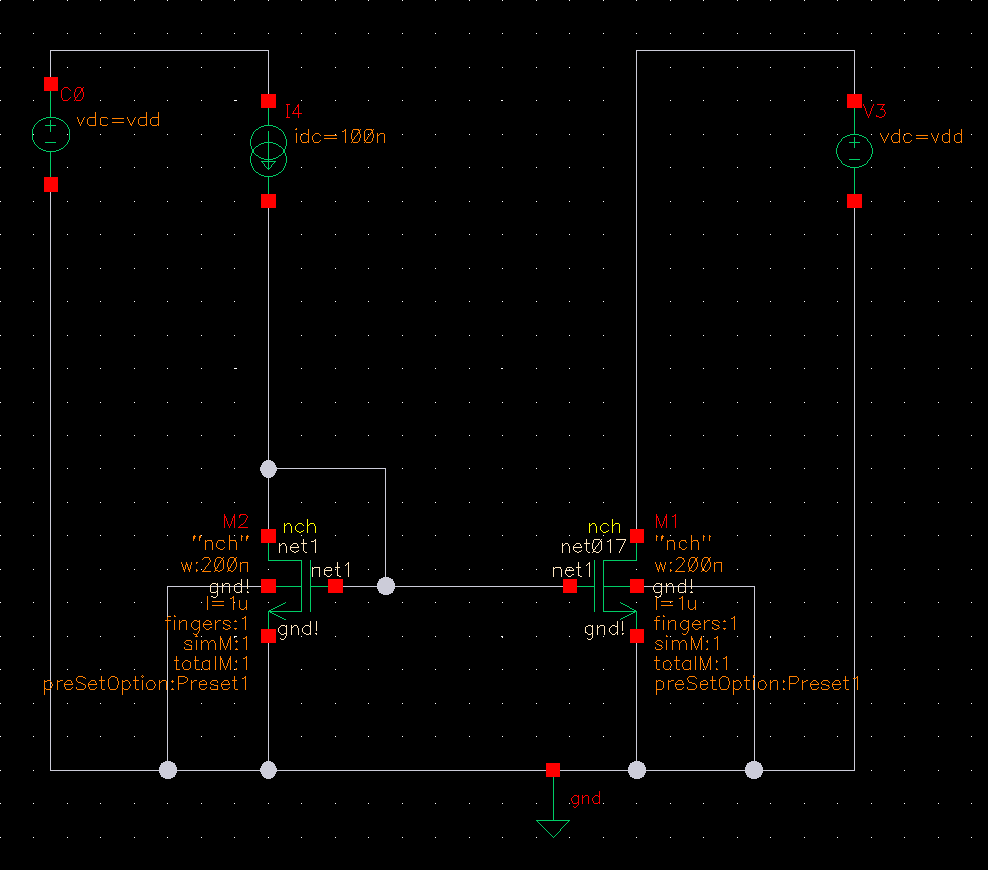
\includegraphics[width=0.8\textwidth]{circuit_d_simple.png}
    \caption{Screencapture of the circuit in figure 1 d) from the lab manual simulated in Cadence.}
    \label{fig:circuitdsimple}
\end{figure}

\begin{figure}[h!]
    \centering
    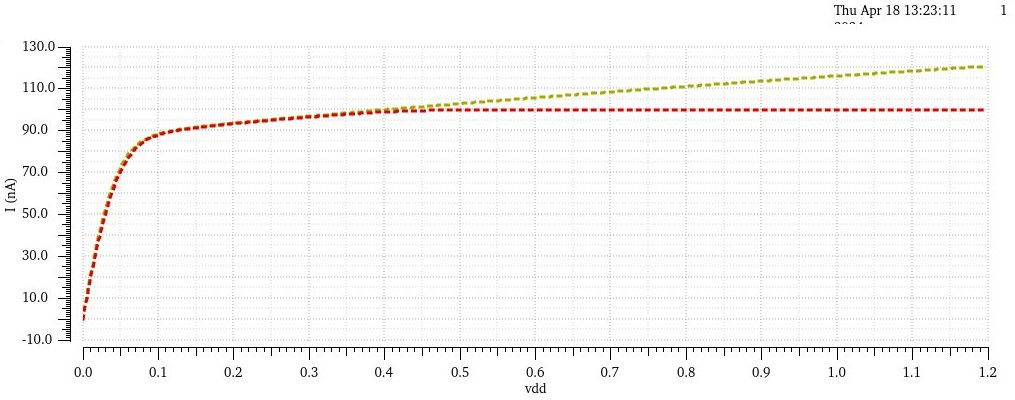
\includegraphics[width=1\textwidth]{plot_circuit_d_dc_sweep_omskjert.jpg}
    \caption{Screencapture of the DC sweep of both circuits in figure 1 d).}
    \label{fig:plotd}
\end{figure}


\end{document}